%\newpage
  \begin{titlepage}
    \vspace*{\fill}
      \part{Feature classification}
    \vspace*{\fill}
  \end{titlepage}

\startcontents[parts]

\phantomsection
\chapter*{Contents}

\textit{This part will focus on the step following feature extraction, which is feature classification. Classification will be introduced in Chapter~\ref{chap:classification}, with a general overview of the classification problem, along with a presentation of some classification algorithms. The last chapter will describe Support Vector Machine classification.} 

\vspace{\baselineskip}

\printcontents[parts]{}{-1}{\setcounter{tocdepth}{1}}

\pagebreak

\phantomsection
\chapter{Classification}
\label{chap:classification}

\noindent Classification is done through machine learning algorithms. Machine learning, being a branch of Artificial Intelligence, aims to helps AI systems improve their performances by learning from their environment. Indeed, the knowledge necessary to build a robust and intelligent system can not always be built-in or explained to it. The solution to this problem is to make the system learn this knowledge through examples and apply it to similar situations. Thus it will be able to perform relevant actions without the need of human intervention. 
\newline

\noindent More specifically, machine learning can be described as a way to develop and implement algorithms taking empirical data as input, and processing these values in order to find links between them. The output will then be used by the system to compute the appropriate action or behaviour. In order to achieve that, the system needs to learn key characteristics from a training dataset given as example or obtained through past experience. It will then study this observable data, and build a model based on it. The system will then use this model to infer actions depending on new data it will get as input.
\newline

\noindent However, machine learning is not only about computing a database and relying on it for every possible situation. In a changing environment, the system needs to know how to learn from these changes and adapt itself.
\newline

\noindent There are many kinds of machine learning algorithms, with their own specificities and level of abstraction. In this chapter we will focus on algorithms behaving like functions and performing pattern recognition. Indeed, a facial image is a set of patterns of different sizes and shapes. Pattern recognition through machine learning can be divided into two main categories of algorithms: supervised learning and unsupervised learning. Those two categories will be described further in this chapter, along with examples.
\newline

\noindent This chapter serves as an introduction for Chapter \ref{chap:svm}, which is about Support Vector Machines, a specific kind of supervised learning algorithm which will be used in our system.
\newline

\phantomsection
\section{Supervised learning}

\vspace{\baselineskip}
\noindent Supervised learning is the task of providing labelled input data to the algorithm, also called \textit{train data}. The main point is that the model is only defined by the observable data it gets for training. It does not make any assumption about underlying, latent variables that could interfere with this observable data. It can then search for patterns and relations between the data points, and build a model fitting these relations before classifying test data.
\newline

\noindent Classification can be divided in two steps, first step being training, and second step being prediction. There are many kinds of supervised learning algorithms, the basic one being a naive Bayes classifier, which will be detailed afterwards. An other example of algorithm is linear discriminant analysis (LDA). Furthermore, the next chapter will focus on an other supervised learning algorithm: Support Vector Machine.
\newline

\subsection{Naive Bayes classifier}

\vspace{\baselineskip}
\noindent The Bayesian classifier is based on Bayes theorem:
\newline

\begin{equation}
    \begin{array}{ll}
        \text{\textbf{sum rule: }} & p(X) = \sum\limits_{Y} p(X,Y) \\
        \text{\textbf{product rule:}} & p(X,Y) = p(Y|X)p(X)
    \end{array}
    \label{bayes}
\end{equation}

\vspace{\baselineskip}
\noindent With these rules, it is possible to compute the \textit{posterior probability} of an event $C_i$ given observable data $x$, using formula \ref{posterior}.

\begin{equation}
	p(C_i|x) = \frac{p(x|C_i \times p(C_i)}{p(x)}
	\label{posterior}
\end{equation}

\noindent With:
\begin{itemize}
\item $p(x|C_i)$ the probability of observed data $x$ given $C_i$, which can also be called the \textit{likelihood function of $C_i$};
\item $p(C_i)$ the prior probability of $C_i$;
\item $p(x)$ the probability of observable data $x$.
\end{itemize} 

\noindent When combined with Bayes theorem, equation \ref{posterior} becomes:

\begin{equation}
	p(C_i|x) = \frac{p(x|C_i \times p(C_i)}{\sum\limits_{k=1}\limits^{K} p(C_k) \times p(x|C_k)}
	\label{posterior_bayes}
\end{equation}

\noindent The classifier output will then be class $C_i$ which meets condition $p(C_i|x) = \max \limits_{k} p(C_k|x)$ (the likelihood function has to be the highest among all classes $C_k$).

\subsection{Linear Discrimination}

\vspace{\baselineskip}
\noindent Since classification is the process of assigning the input vector $x$ to one of the classes $C_i$, $i=1, ..., I$, its key point is about learning the decision boundaries that separate the different classes in the input space \cite{BIS06}. If the input dataset is \textit{linearly separable}, decision boundaries can then be described by linear functions of the input vector $x$.
\newline

\noindent For example, the linear discriminant function for a 2-class problem will look like 

\begin{equation}
y(x) = w^Tx + \omega_0
\end{equation}

\noindent With \textit{weight vector} $w^T$ and \textit{bias} $\omega_0$ \cite{BIS06}. The input vector $x$ is then assigned to class $C_1$ if $y(x) = 0$, otherwise it will be classified as belonging to class $C_2$.
\newline

\noindent For problems with a number of classes K > 2, a \textit{one-versus-the-rest} approach can be used, where K-1 two-way discriminant functions are used: the $k^{th}$ discriminant function will determine if a point belongs to class $C_k$ or not. However, as shown in Figure \ref{one_vs_rest}, this combination of discriminant functions leaves an ambiguous region \cite{BIS06}. 
\newline

\begin{figure}[!h]
\begin{center}
\noindent 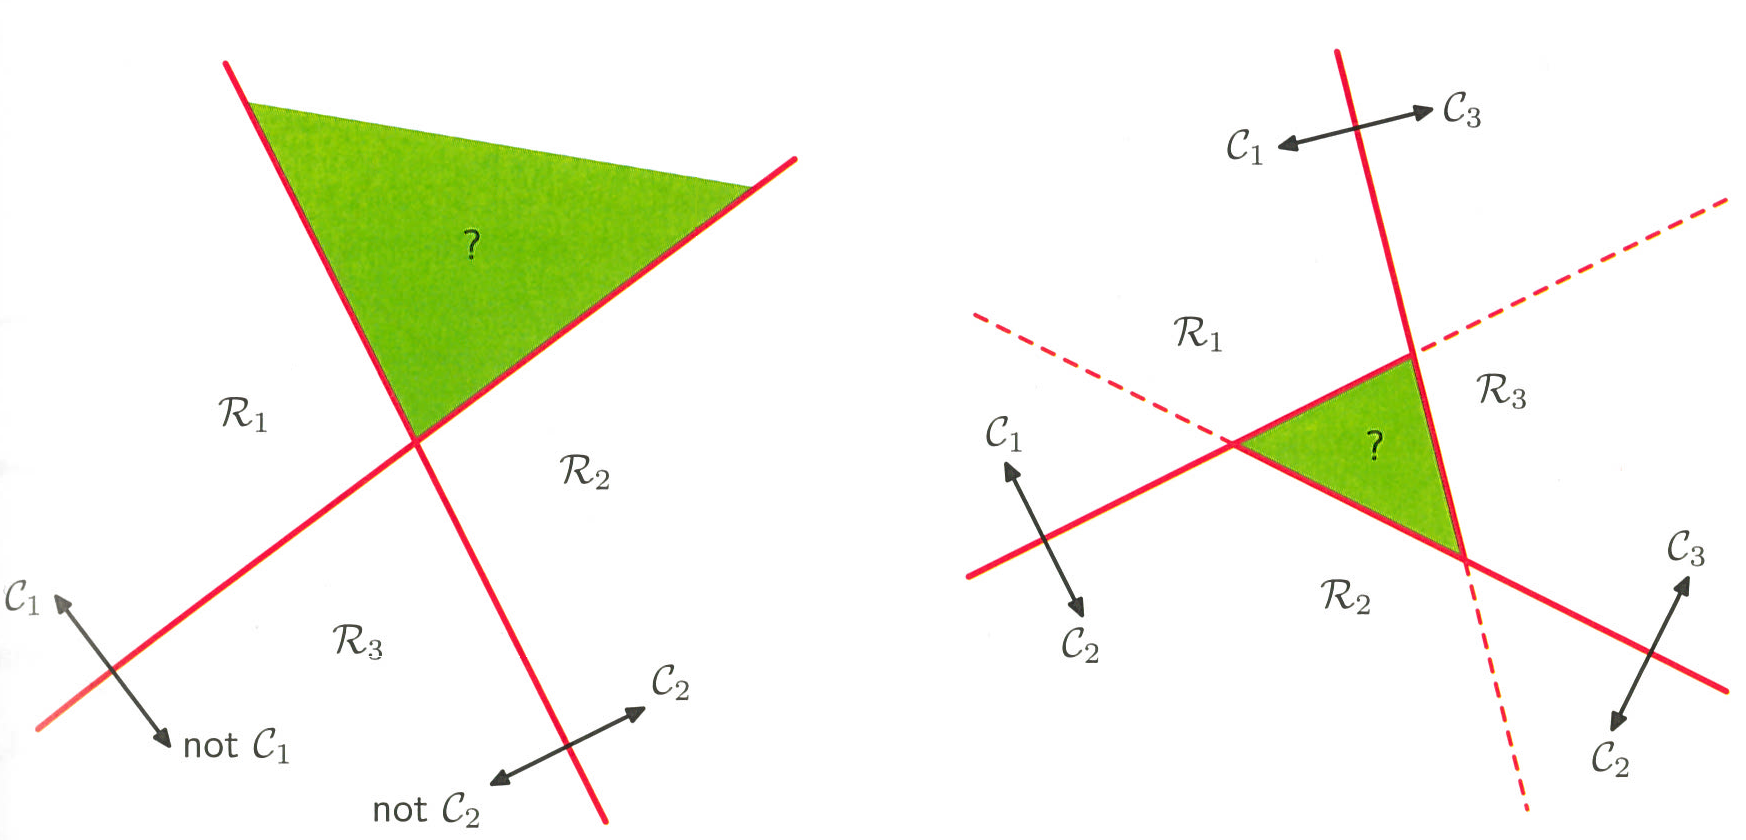
\includegraphics[scale=0.2]{figures/one_vs} 
\newline
\caption{Attempting to construct a $K$ class discriminant from a set of two class discriminants leads to ambiguous regions, shown in green. On the left is an example of \textit{one-versus-the-rest} approach, the discriminant function designed to separate points belonging to a class $C_i$ and points that are not. On the right is an example of \textit{one-versus-all} approach involving 3 discriminant functions, each one separating a pair of classes classes $C_i$ and $C_j$.From: Christopher M. Bishop, \textit{Pattern Recognition and Machine Learning}. Copyright \copyright  2006 by Springer Science.}
\label{one_vs_rest}
\end{center} 
\end{figure}

\noindent An other way to solve a multi-class problem could be to use $\frac{K(K-1)}{2}$ discriminant functions, which is the \textit{one-versus-all} approach. However, the resulting K-class discriminant also has an ambiguous region problem, as seen in Figure \ref{one_vs} \cite{BIS06}.
\newline

\noindent A K-class discriminant which does not lead to an ambiguous region problem is to use K linear discriminant functions $g(x)_k$, $k=1..K$, and to assign an input vector $x$ to a class $C_i$ if $g(x)_i = \max\limits_{k} g_k(x)$. Indeed, as shown in Figure \ref{k_discr}, there are no more ambiguous regions \cite{BIS06}.
\newline

\begin{figure}[!h]
\begin{center}
\noindent 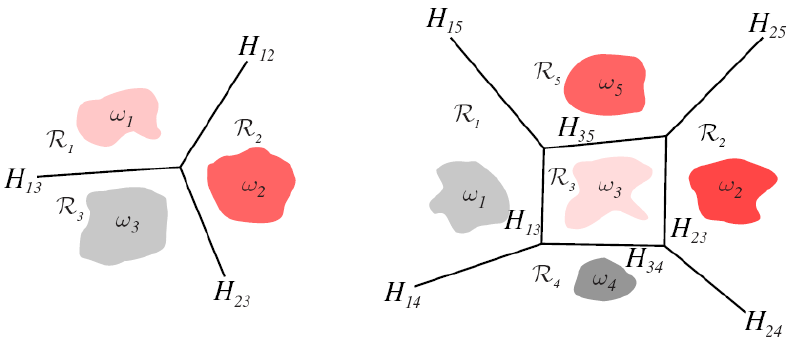
\includegraphics[scale=0.5]{figures/lda_k_disc} 
\newline
\caption{Decision boundaries produced by a linear machine for a 3-class problem and a 5-class problem. From: Richard O. Duda, Peter E. Hart, and David G. Stork, \textit{Pattern Classification}. Copyright \copyright  2001 by John Wiley \& Sons Inc.}
\label{k_disc}
\end{center} 
\end{figure}

\phantomsection
\section{Unsupervised learning}

\vspace{\baselineskip}
\noindent Unlike supervised learning, the classification algorithm is not fed with train data in the case of unsupervised learning. It will be given a set of observable data, and its goal is to group data the smartest way possible, and by itself. Furthermore, in unsupervised learning, the concept of \textit{class} is not applicable any more; the term \textit{cluster} being preferred.
\newline

\noindent The key point of unsupervised algorithms is data clustering. In most common unsupervised algorithms such as K-means, the algorithm can get a hint of the number of clusters it has to find. It then proceeds, usually in an iterative way, to find the latent variables related to the data. Indeed, it is assumed that all observable data is governed by latent variables which can be organized in different levels.
\newline

\noindent Besides K-means, an other common unsupervised algorithm is the Mixture Models algorithm, which will also be described in the following subsections.
\newline

\subsection{K-Means}

\vspace{\baselineskip}
\noindent K-means clustering relies on a set of k reference vectors $\mu_k$, $k=1..K$, also called \textit{prototype vectors}. These vectors represent the centres of the K clusters. This clustering method has two goals: first, it has to find how the clusters are shaped and which data lies in which cluster; secondly, the set of vectors $\{\mu_k\}$ has to be determined while verifying the following condition: for each data point $x_n$, the sum of squares of the distances between $x_n$ and its closest vector $\mu_k$ is a minimum. In other words, equation \ref{distort_fc}, also called \textit{distortion function} has to be minimized \cite{BIS06}.

\begin{equation}
J = \sum\limits_{n=1}\limits^{N} \sum\limits_{k=1}\limits^{K} r_{nk} ||x_n - \mu_k||^2
\label{distort_fc}
\end{equation}

\noindent With

\begin{equation*}
r_{nk} = \left\{
	\begin{array}{ll}
		1 & \mbox{if }  k = arg \min_j ||x_n - \mu_j||^2 \\
		0 & \mbox{otherwise}
	\end{array}
\right.
\end{equation*}
\vspace{\baselineskip}

\noindent This can be achieved through the following iterative algorithm, which result can be seen in Figure \ref{k-mean_res}:
\newline

\begin{algorithmic}
\State Initialization of reference vectors $\mu_k$, $k = 1..K$ 
\Repeat	
	\ForAll{$x_n \in \chi$}
		\State \begin{math} 
			r_{nk} \gets \left\{
			\begin{array}{ll}
				1 & \mbox{if }  k = arg \min_j ||x_n - \mu_j||^2 \\
				0 & \mbox{otherwise}
			\end{array}
			\right.
			\end{math}
	\EndFor
	\ForAll{$\mu_k$, $k = 1..K$ }
		\State $\mu_k \gets \frac{\sum\limits_n r_{nk}x_n}{\sum\limits_n r_{nk}}$
	\EndFor
\Until{$\mu_k$ converge}
\end{algorithmic}

\vspace{\baselineskip}

\begin{figure}[!h]
\begin{center}
\noindent 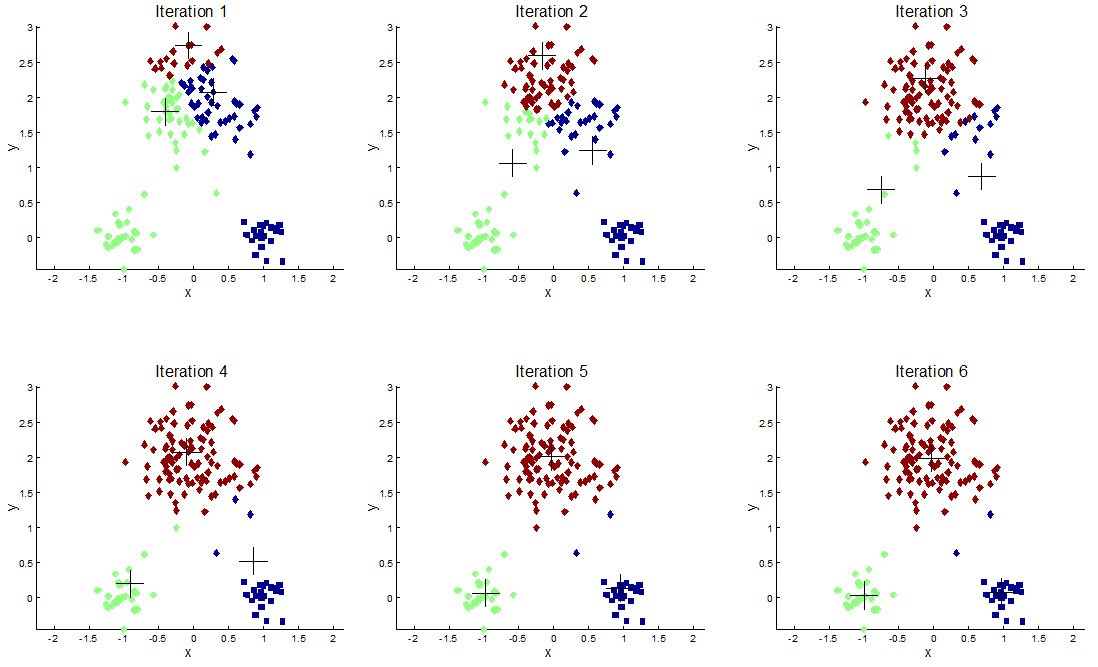
\includegraphics[scale=0.5]{figures/k-mean_res} 
\newline
\caption{Example of application of the iterative K-means algorithm.}
\label{k-mean_res}
\end{center} 
\end{figure}

\noindent In this algorithm, denominator $\sum\limits_n r_{nk}$ corresponds to the number of points assigned to cluster $k$, which sets $\mu_k$ as the mean of the cluster, hence the name \textit{K-means algorithm} \cite{BIS06}.
\newline

\noindent This algorithm can also be used in \textit{lossy data compression}, where input data can be reconstructed with minor errors, in contrary to \textit{lossless data compression}. If the K-means algorithm is applied, then for each data point $x_n$ the only value stored is the cluster $k$ it belongs to. Apart from the data points, values of cluster centres $\mu_k$ are also stored. Hence, during data reconstruction, each data point is approximated by corresponding vector $\mu_k$. This approximation is called \textit{vector quantization} \cite{BIS06}.
\newline

\subsection{Mixture of Gaussians}

\vspace{\baselineskip}
\noindent While the K-means algorithm will try to find reference vectors describing the different clusters, the mixture models algorithm will rather model the underlying distribution of the clusters, usually by a Gaussian probability density function. Each cluster is then represented by a Gaussian distribution, and the aim of the algorithm is to find the best parameters for the latent variables governing these distributions. It can be achieved by finding parameters maximizing likelihood $p(x)=p(x|G_i)p(G_i)$, with:

\begin{itemize}
\item $G_i$: clusters
\item $p(G_i)$: prior probability (mixture proportion)
\item $p(x|G_i)$: component density
\end{itemize}

\noindent Since a Gaussian mixture is roughly similar to $p(x|G_i) \sim \mathcal{N}(\mu_i, \Sigma_i)$, with mean vector $\mu_i$ and covariance matrix $\Sigma_i$, the goal is now to maximize the log likelihood function described in Equation \ref{log_likelihood}.

\begin{equation}
\begin{array}{ll}
\mathcal{L}(\Phi|\chi) & = \ln \prod\limits_n p(x^n | \Phi) \\
 & = \sum\limits_{n=1}\limits^{N} \left\{ \sum \limits_{k=1}\limits^{K} \pi_k \mathcal{N}(x_n|\mu_k, \Sigma_k)\right\}
\end{array}
\label{log_likelihood}
\end{equation}

\noindent with $\Phi$ representing mixing coefficients, including prior probabilities and sufficient statistics of component densities.
\newline

\noindent The maximum likelihood estimation can then be obtained through the \textit{Expectation-Maximization algorithm} for Gaussian Mixture Models (EM), which converges into a result comparable as the one in Figure \ref{mixture_model} \cite{BIS06}.
\newline

\noindent \textbf{Expectation-Maximization algorithm:}
\newline

\begin{algorithmic}
\State Initialize means $\mu_n$, covariances $\Sigma_n$, mixing coefficients $\pi_n$ and compute initial value of the log likelihood

\Repeat
	\State \textbf{Expectation step}: Evaluate the expected value of the latent variable using current parameter values:
		\State $\gamma(z_{nk}) = 
		\frac{\pi_k\mathcal{N}(x_n|\mu_k, \Sigma_k)}{\sum\limits_{j=1}\limits^{K}\pi_j\mathcal{N}(x_n|\mu_j, \Sigma_j)}$
	\State \textbf{Maximization step}: Re-estimate the parameters using $\gamma(z_{nk})$:
		\State $\pi^{new}_k = \frac{N_k}{N}$
		\State $\mu^{new}_k = \frac{1}{N_k}\sum\limits_{n=1}\limits{N}\gamma(z_{nk})x_n$
		\State $\Sigma^{new}_k = \frac{1}{N_k}\sum\limits_{n=1}\limits{N}\gamma(z_{nk}) (x_n - \mu^{new}_k) (x_n - \mu^{new}_k)^T$
		\State Where $N_k = \sum\limits_{n=1}\limits{N}\gamma(z_{nk})$
	\State Evaluate log likelihood $\mathcal{L}$ 
\Until {$\mathcal{L}$ converges}
\end{algorithmic}

\begin{figure}[!h]
\begin{center}
\noindent 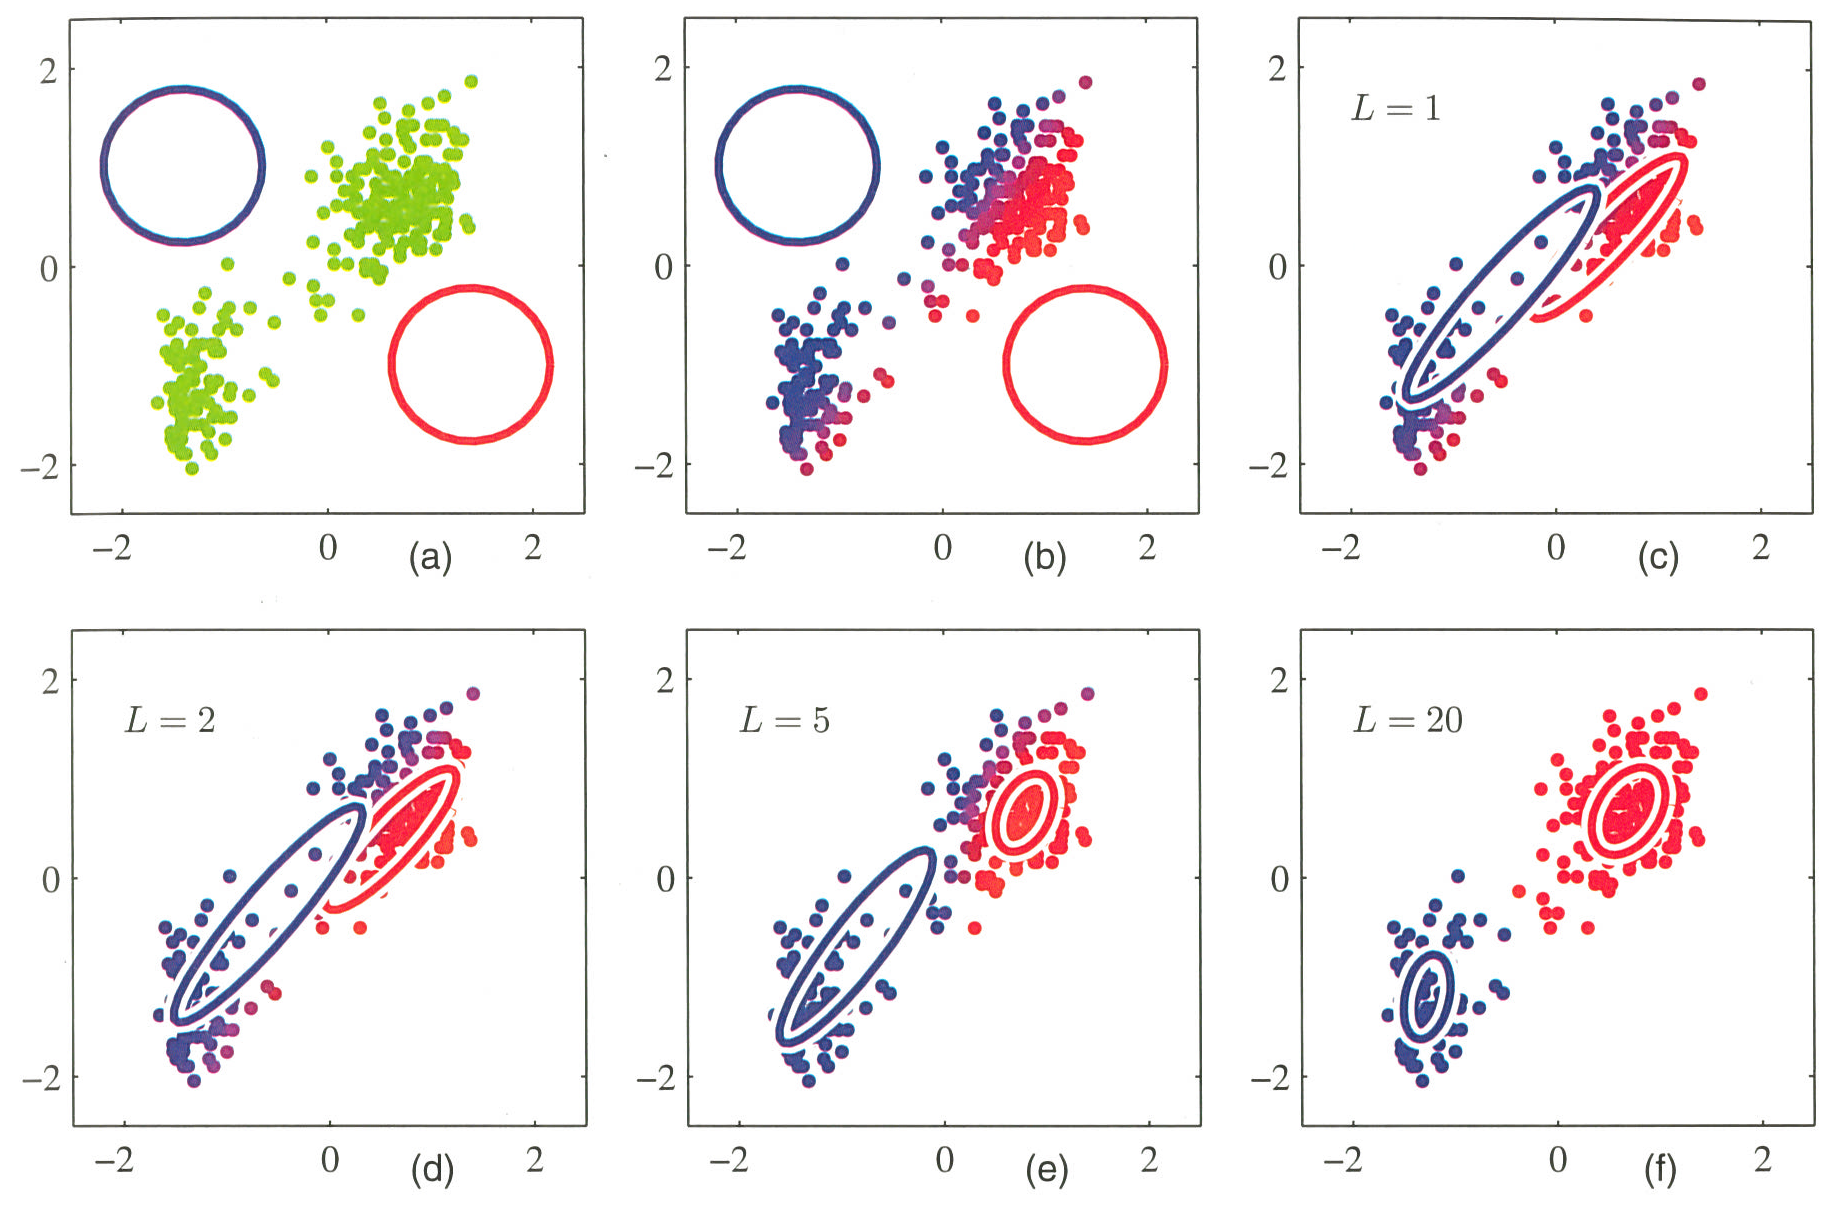
\includegraphics[scale=0.2]{figures/mixture_model} 
\newline
\caption{Illustration of the EM algorithm. From: Christopher M. Bishop, \textit{Pattern Recognition and Machine Learning}. Copyright \copyright  2006 by Springer Science.}
\label{mixture_model}
\end{center} 
\end{figure}
\pagebreak

\clearpage
\newpage
\phantomsection
\chapter{Support Vector Machine}
\label{chap:svm}

\noindent Support Vector Machine (SVM) is a binary linear classifier belonging to the supervised learning algorithms category. It has been proven to be very efficient for classification, regression and novelty detection problems \cite{BIS06}, which makes it suitable for facial expression recognition.
\newline

\noindent This chapter will first provide an overview of how classification is performed using SVM. It will then focus and describe the key points behind this classifier, namely \textit{margin maximization} and \textit{kernel function}. The chapter will conclude with the review of a research paper detailing facial expression recognition using LBP for feature extraction and SVM for classification.
\newline

\phantomsection
\section{Overview}
\label{svm_overview}

\vspace{\baselineskip}
\noindent SVM is originally a binary classifier, which means it has a \textit{one-vs-all} approach. It is a decision machine, so its output is not a posterior probability, but rather a class label \cite{BIS06}.  It can be adapted into a \textit{relevance vector machine} to output posterior probabilities though \cite{BIS06}, but this alternative will not be detailed in our report.
\newline

\noindent SVM is also a linear classifier, such as LDA. For a two-class problem, it will linearly separate the train data by finding the optimal hyperplane between these 2 classes. This hyperplane is defined as being as far as possible from both classes. \textit{Margin maximization} is then applied to optimize the distance between the two classes and the hyperplane, as it will be explained in Section \ref{margin_max}.
\newline

\noindent The name "Support Vector" originates from the margin maximization feature. Indeed, the distance between the classes and the separating hyperplane is computed regarding to the closest data points from both classes. These particular data points, lying on the margins edges, are the support vectors. Some properties are associated to these vectors, such as non-zero Lagrange multipliers (see Section \ref{margin_max}), which builds the classification algorithm.
\newline

\noindent For a multi-class problem, however, this linear separation is not possible anymore. The dataset has to be mapped into an other space, where it can be linearly separated. This is what \textit{kernel functions} are used for, as described in Section \ref{kernel_fct}.
\newline

\phantomsection
\section{Margin maximization}
\label{margin_max}

\vspace{\baselineskip}
\noindent As introduced in Section \ref{svm_overview}, margin maximization for a two-class linear problem starts by finding the separating hyperplane between these two classes. A linear classification model of the form $f(x) = w(x) + b$ can be inferred, with $w$ being the normal to the hyperplane and $b$ the bias. The hyperplane can then be characterized by  $w(x) + b = 0$.
\newline

\noindent Margin is defined as the distance between the closest point of the class to the hyperplane, and that hyperplane, which can also be written as $ d(x) = \frac{|w(x) + b |}{||w||}$. Since a data point $(x_i, y_i)$ is correctly classified if $yf(x) \geq 1$, maximizing the margin is the action of maximizing $||w||^{-1}$, which is consequently equivalent to minimizing $||w||^2$ depending on this constraint. Margin maximization then requires to solve a \textit{quadratic programming} problem under constraints, as seen in Equation \ref{margin_max_eq}.

\begin{equation}
\left\{
\begin{array}{l}
\min \frac{1}{2} ||w||^2 \\
\forall i, \, y_i . f(x) \geq 1
\end{array}
\right.
\label{margin_max_eq}
\end{equation}

\vspace{\baselineskip}

\phantomsection
\section{Kernel function}
\label{kernel_fct}

\vspace{\baselineskip}
\noindent It might however not be possible to perform this linear separation with more classes. Indeed, data might be overlapping, and thus it will not be a linear problem anymore. The solution to overcome this problem is to map the non-linear dataset from its input space into a higher feature space using a function $\Phi(x)$, and perform margin maximization and classification in this higher space. 
\newline

\noindent In order to achieve this mapping, a \textit{kernel function} of the form $K(x_i, x_j) = \Phi(x_i)^T \Phi(x_j)$ is applied to the dataset. This kernel represents an inner product in the feature space. There are four kernels available, which are described in Equation \ref{kernels_svm}.
\newline

\begin{equation}
\begin{array}{ll}
	\text{Linear kernel:} & K(x_i,x_j) = x_i^Tx \\
	\text{Polynomial kernel:} & K(x_i,x_j) = (\gamma x_i^Tx_j + r)^T, \gamma > 0 \\
	\text{Radial Basis Function (Gaussian) kernel:} & K(x_i,x_j) = \exp(-\gamma \| x_i - x_j \|^2), \gamma > 0 \\
	\text{Sigmoid kernel:} & K(x_i,x_j) = \tanh(\gamma x_i^T x_j + r)\\
\end{array}
\label{kernels_svm}
\end{equation}

\noindent The main advantage of using a kernel function is that there is no need to define or calculate $\Phi(x_i)$, only $\Phi(x_i)^T \Phi(x_j)$. We hence do not know the true form of $\Phi(x_i)$. However, simple kernels are usually combined in order to build more complex ones.
\newline

\phantomsection
\section{Combining LBP and SVM}

\vspace{\baselineskip}
\noindent In a 2009 article, Shang and al \cite{SHA09} have performed facial expression recognition while using Local Binary Patterns for feature extraction, and comparing the accuracy of different kinds of classifiers:  template matching,  LDA and SVM. They have used images from the Cohn-Kanade database as train data, and the conclusion of their study is that classification using SVM has a high accuracy rate, as seen in Table \ref{accuracy_svm_lbp}. 
\newline

\begin{table}[h]
   \caption{\label{accuracy_svm_lbp} Recognition performance of LBP-based SVM with different kernels}
\begin{tabular}{|lcc|}
\hline
 & 6-Class recognition (\%) &  7-Class recognition (\%) \\
 \hline
 SVM (linear) & 91.5 $\pm$ 3.1 & 88.1 $\pm$ 3.8 \\
 SVM (polynomial) & 91.5 $\pm$ 3.1 & 88.1 $\pm$ 3.8 \\
 SVM (RBF) & 92.6 $\pm$ 3.1 & 88.9 $\pm$ 3.5 \\
 \hline
\end{tabular}
\end{table}

\noindent Furthermore, as seen in confusion matrices \ref{conf_mtx_6_svm_lbp} and \ref{conf_mtx_7_svm_lbp}, the accuracy for each facial expression is not the same. SVM has some difficulties especially when it comes to distinguish fear and sadness, the two facial expressions which have the lowest accuracy rates. Fear is mistaken with joy, while sadness is mistaken with anger or neutral state. Recognitions rates are however usually better for a 7-class classification, except for fear.
\newline

\noindent Since the accuracy of the system presented in this article is very high, we chose to implement a similar system. Indeed, we are performing facial expression recognition using LBP for feature extraction, and SVM classification. We however did not use the Cohn-Kanade database as train data. We will describe further our implementation and results further in the report. 
\newline

\begin{table}[h]
\caption{\label{conf_mtx_6_svm_lbp} Confusion matrix of 6-class facial expression recognition using SVM (RBF)}
\begin{tabular}{|lcccccc|}
\hline
 & Anger (\%) & Disgust (\%) & Fear (\%) & Joy (\%) & Sadness (\%) & Surprise (\%) \\
\hline
Anger & 89.7 & 2.7 & 0 & 0 & 7.6 & 0 \\
Disgust & 0 & 97.5 & 2.5 & 0 & 0 & 0 \\
Fear & 0 & 2.0 & 73.0 & 22.0 & 3.0 & 0 \\
Joy & 0 & 0.4 & 0.7 & 97.9 & 1.0 & 0 \\
Sadness & 10.3 & 0 & 0.8 & 0.8 & 83.5 & 4.6 \\
Surprise & 0 & 0 & 1.3 & 0 & 0 & 98.7 \\
\hline
\end{tabular}
\end{table}

\begin{table}[h]
\caption{\label{conf_mtx_7_svm_lbp} Confusion matrix of 7-class facial expression recognition using SVM (RBF)}
\begin{tabular}{|lccccccc|}
\hline
& Anger (\%) & Disgust (\%) & Fear (\%) & Joy (\%) & Sadness (\%) & Surprise (\%) & Neutral (\%) \\
\hline
Anger & 85.0 & 2.7 & 0 & 0 & 4.8 & 0 & 7.5 \\
Disgust & 0 & 97.5 & 2.5 & 0 & 0 & 0 & 0 \\
Fear & 0 & 2.0 & 68.0 & 22.0 & 1.0 & 0 & 7.0 \\
Joy & 0 & 0 & 0.7 & 94.7  & 1.1 & 0 & 3.5 \\
Sadness & 8.6 & 0 & 0 & 0 & 69.5 & 2.3 & 19.6 \\
Surprise & 0 & 0 & 1.3 & 0 & 0 & 98.2 & 0.5 \\
Neutral & 1.6 & 0.4 & 0 & 1.6 & 6.0 & 0.4 & 90.0 \\
\hline
\end{tabular}
\end{table}


\stopcontents[parts]


